\documentclass{book}
\usepackage{geometry}
\geometry{
 a4paper,
 total={170mm,257mm},
 left=20mm,
 top=20mm,
 }
\usepackage[french]{babel}
\usepackage[T1]{fontenc}
\usepackage[utf8]{inputenc}
\usepackage{lmodern}
\usepackage{graphicx}
\usepackage{amssymb}
\usepackage{microtype}
\usepackage[colorlinks=true,
            linkcolor=red,
            urlcolor=blue,
            citecolor=blue]{hyperref}
            
\title{Simulation de fluides}
\author{Raoelisolonarivony - MISA M2}
\date{Juillet 2017}

\setlength{\parindent}{2em}
\setlength{\parskip}{1em}
\linespread{1.3}
\usepackage{fancyhdr}
\pagestyle{fancy}

\renewcommand{\headrulewidth}{0.5pt}
\fancyhead[L]{RAOELISOLONARIVONY - MISA M2 - \textit{Simulation de fluides}}
\fancyhead[C]{}
\fancyhead[R]{Juillet 2017}

\graphicspath{ {images/} }

\begin{document}

\maketitle

\begin{center}
  
\includegraphics[scale=0.25]{001_logo_univ_tana}
  
\includegraphics[scale=0.25]{002_logo_fac_sciences}
  
\includegraphics[scale=0.25]{003_logo_dmi}
  
\includegraphics[scale=0.25]{004_logo_misa}
  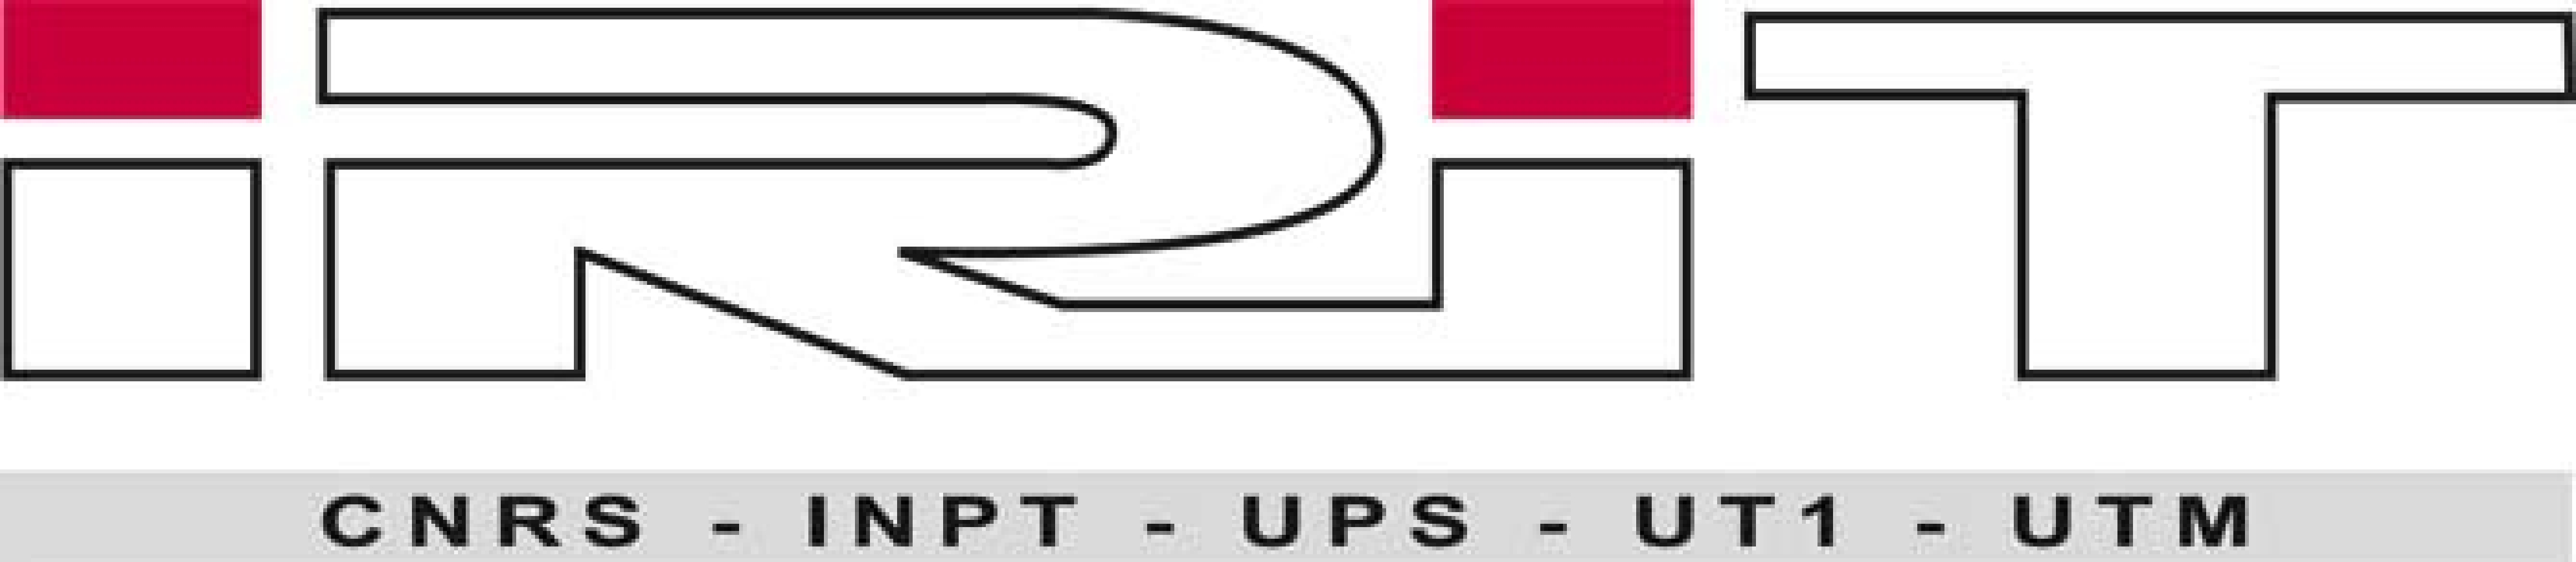
\includegraphics[scale=0.125]{005_logo_irit}
  
\includegraphics[scale=0.0425]{006_logo_univ_toulouse}
\end{center}

\end{document}